\documentclass[journal]{IEEEtran}
\usepackage[a5paper, margin=10mm, onecolumn]{geometry}
\usepackage{lmodern} % Ensure lmodern is loaded for pdflatex
\usepackage{tfrupee} % Include tfrupee package

\setlength{\headheight}{1cm} % Set the height of the header box
\setlength{\headsep}{0mm}     % Set the distance between the header box and the top of the text

\usepackage{gvv-book}
\usepackage{gvv}
\usepackage{cite}
\usepackage{amsmath,amssymb,amsfonts,amsthm}
\usepackage{algorithmic}
\usepackage{graphicx}
\usepackage{textcomp}
\usepackage{xcolor}
\usepackage{txfonts}
\usepackage{listings}
\usepackage{enumitem}
\usepackage{mathtools}
\usepackage{gensymb}
\usepackage{comment}
\usepackage[breaklinks=true]{hyperref}
\usepackage{tkz-euclide} 
\usepackage{listings}                                      
\def\inputGnumericTable{}                                
\usepackage[latin1]{inputenc}                                
\usepackage{color}                                            
\usepackage{array}                                            
\usepackage{longtable}
\usepackage{multicol}
\usepackage{calc}                                            
\usepackage{multirow}                                        
\usepackage{hhline}                                          
\usepackage{ifthen}                                          
\usepackage{lscape}
\begin{document}

\bibliographystyle{IEEEtran}
\vspace{3cm}

\title{9.6.16}
\author{EE24BTECH11004 - ANKIT JAINAR}
{\let\newpage\relax\maketitle}

\renewcommand{\thefigure}{\theenumi}
\renewcommand{\thetable}{\theenumi}
\setlength{\intextsep}{10pt} % Space between text and floats

\numberwithin{equation}{enumi}
\numberwithin{figure}{enumi}
\renewcommand{\thetable}{\theenumi}

\textbf{Question}:
Find the equation of a curve passing through the origin, given that the slope of the tangent to the curve at any point $(x, y)$ is equal to the sum of the coordinates of the point.
\newline
\textbf{Solution:}
\newline
\begin{table}[h!]    
  \centering
  \begin{tabular}[12pt]{ |c| c| c |}
    \hline
    \textbf{Variable} & \textbf{Description} & \textbf{values}\\ 
    \hline
    $\vec{V}$ & Quadratic form of the matrix & $\myvec{1 & 0 \\ 0 & 1} $\\
    \hline
    $\vec{u}$ & Linear coefficient vector & $\myvec{0 \\ 0} $\\
    \hline
    f & constant term & -4 \\ 
    \hline
    $\vec{m}$ & The direction vector of line & $\myvec{1 \\ 0}$\\
    \hline
     $\vec{h}$ & Point on line & \myvec{2 \\ 0} \\
     \hline
\end{tabular}

  \label{tab1.1.2.2}
\end{table}
\newline
\textbf{Theoretical Solution:}
\newline
Given:
\begin{align}
    \frac{dy}{dx} &= x + y
\end{align}
This is a first-order linear differential equation. Rewriting:
\begin{align}
    \frac{dy}{dx} - y &= x
\end{align}
\newline
Using the integrating factor:
\begin{align}
    \text{IF} &= e^{\int -1 dx} = e^{-x}
\end{align}
Multiplying through by the integrating factor:
\begin{align}
    e^{-x} \frac{dy}{dx} - e^{-x}y &= xe^{-x} \\
    \frac{d}{dx}\left(e^{-x}y\right) &= xe^{-x}
\end{align}
\newline
Integrating both sides:
\begin{align}
    e^{-x}y &= \int xe^{-x} dx
\end{align}
Using integration by parts:
\begin{align}
    \int xe^{-x} dx &= -xe^{-x} + \int e^{-x} dx \\
    &= -xe^{-x} - e^{-x}
\end{align}
Thus:
\begin{align}
    e^{-x}y &= -xe^{-x} - e^{-x} + C
\end{align}
Multiply through by $e^x$:
\begin{align}
    y &= -x - 1 + Ce^x
\end{align}
\newline
Applying the initial condition $y(0) = 0$:
\begin{align}
    0 &= -0 - 1 + C \cdot e^0 \implies C = 1
\end{align}
Therefore, the solution is:
\begin{align}
    y &= -x - 1 + e^x
\end{align}
\newline
\textbf{Computational Solution:}

Given:
\begin{align}
    \frac{dy}{dx} &= x + y
\end{align}
Using the discretized form:
\begin{align}
    y_{n+1} = y_n + h(x_n + y_n)
\end{align}
Where $h$ is the step size. Starting with $x_0 = 0$, $y_0 = 0$, compute $y$ at successive points. 
\newline
By iterating over the time steps, the computational solution is computed. A comparison of theoretical and computational results is shown below.
\newline
\begin{figure}[h!]
   \centering
   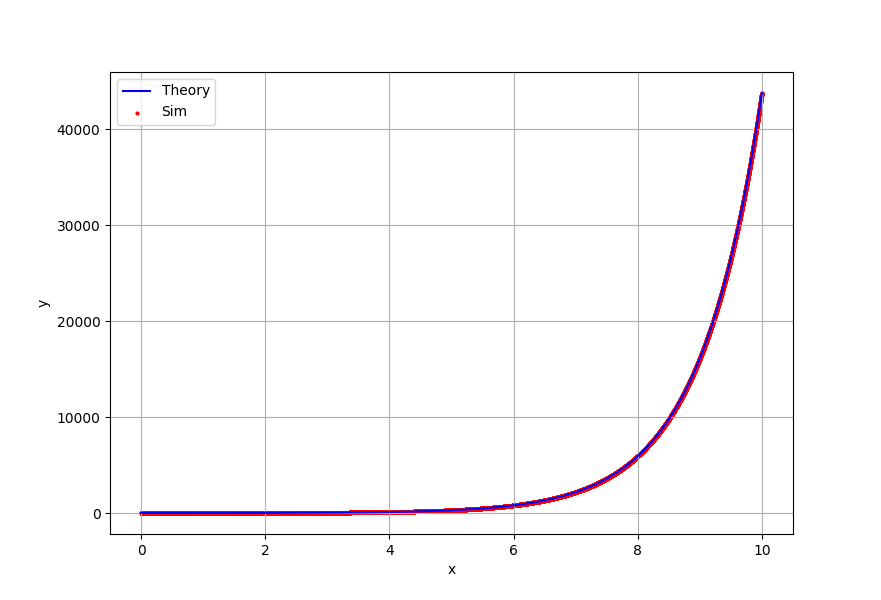
\includegraphics[width=\columnwidth]{fig/fig.png}
   \label{comparison}
\end{figure}
\newline
\end{document}

